\documentclass[a4paper,12pt]{texMemo}
\usepackage[english]{babel}
\memoto{Patrick Peters}
\memofrom{Steven Hill}
\memosubject{Progress Report}
\memodate{\today}


\usepackage{rotating}
\usepackage{indentfirst}
\usepackage{lineno}
\usepackage{fancyhdr}
\pagestyle{fancy}
\usepackage[utf8]{inputenc}
\usepackage{amsmath}
\usepackage{amsfonts}
\usepackage{amssymb}
\usepackage{graphicx}
\usepackage{setspace}
\usepackage{outline}
\newcommand{\bibent}{\noindent \hangindent 40pt}
\newenvironment{workscited}{ \doublespacing \newpage \begin{center} Works Cited \end{center}}{\newpage }

\begin{document}
\maketitle

\section{Progress Report}
The project I am working on is on the development of technical documentation for Easy-Terminal-Alternative as the Center for Genome Research and Biocomputing. This includes an overview of the software, it's purpose, the need for the software, the systems architecture, the way it is configured to work on the CGRB's infrastructure, installation, and the developer documentation for the software. 

The project progress so far has been slow. The only work done is what will be seen in this progress report. The last week was spent almost entirely finishing my senior design project in preparation for the engineering expo. However, the project is still mostly meeting the schedule outlined in the proposal.

An interview with Chris Sullivan, lead computational scientist at the Center for Genome Research and Biocomputing has been scheduled for Thursday. The UML diagrams as listed are not all completed. The Package overview diagram has been finished, but the dataflow diagram is not finished. I am planning on generating the class UML diagrams, but these may prove to be too large to be included. 

Additionally, the architecture section still needs the dataflow writeup itself and a description of the environment that Easy-Terminal-Alternative lives in at the CGRB. The other sections still need to be written and the java-docs need to be created.

Throughout the next week I will continue to add sections to the first draft and meet the listed schedule of the 29th. The project itself has been placed in a git repository to maintain version control and a remote backup of the paper.
\newpage

\section{Sample Work}
\subsection{Easy-Terminal-Alternative Architecture}
ETA is built on several preexisting technologies. These technologies are, Java, Google-web-toolkit (GWT), and Apache Tomcat. Java is the programming language used for both the server application and the client application, GWT compiles java  to create the HTML and Javascript that will appear in the users browser, and Tomcat is the webserver which handles all of the requests and the application ultimately lives on.

\subsection{Aspect-Oriented Design}
In order for an application of this magnitude to be modular, it was important that the design included a way to functionally be independent of all other parts of the application. That is, if something broke on the client-side, it would not affect the other parts of the application. The primary design pattern used was an Aspect-Oriented Design. That is, an architecture that is designed around modularity. 

One study concluded that, "AO architectures tended to require less invasive changes" (Molesini et al. 722). Being able to add or modify functionality is imperative for any new technology. For example, if the Center for Genome Research and Biocomputing was to change authentication methods, ETA should be able to adapt to this new method without breaking any other parts of the application. As a result of these needs, ETA was designed with this in mind.

\subsection{Package Overview}
ETA is broken up into many different packages. "Package objects contain version information about the implementation and specification of a Java package" (Java Platform SE 7). The application is into many packages. The following is the package hierarchy:

\begin{enumerate}
    \item client:
    \begin{enumerate}
        \item button
        \item images
        \item pipeline
        \item table
        \item tabs
        \item tabset
        \item tools
        \item window
        \item wrapperrunner
    \end{enumerate}
    \item etadrive
    \begin{enumerate}
        \item desktop
    \end{enumerate}
    \item remote
    \begin{enumerate}
        \item api
    \end{enumerate}
    \item server
    \begin{enumerate}
        \item mysql
        \item remote
        \item rmi
        \item services
        \item settings
    \end{enumerate}
    \item shared
    \begin{enumerate}
        \item etatype
        \item pipeline
        \item wrapper
    \end{enumerate}
\end{enumerate}

Each package servers a purpose and is as decoupled as possible from the other packages. Although complete decoupling is impossible, the higher level classes are written to be as independent as possible. The main coupling that occurs is in the methods that are implemented across the platform, such as client from server, and the remote class from the server. See  \ref{ETAPackageOverview} for detail about the main package relations. 

Inside of each main package, there contains more packages. These are typically reserved for inheritance between similar classes. The most obvious use of this is in the client package. Many different GUI "widgets", or things a user interacts with such as buttons and labels, will often be reused to have different purposes and slightly different appearances. As stated in the official Java API, "Inheritance provides a powerful and natural mechanism for organizing and structuring your software" (Java Platform SE 7).

An important thing to note is that the majority of the work is done in the server package. There are several different "services", or additional programs that ETA relies on which are implemented inside of the server package. This will be expanded on in a later section.
\begin{figure}
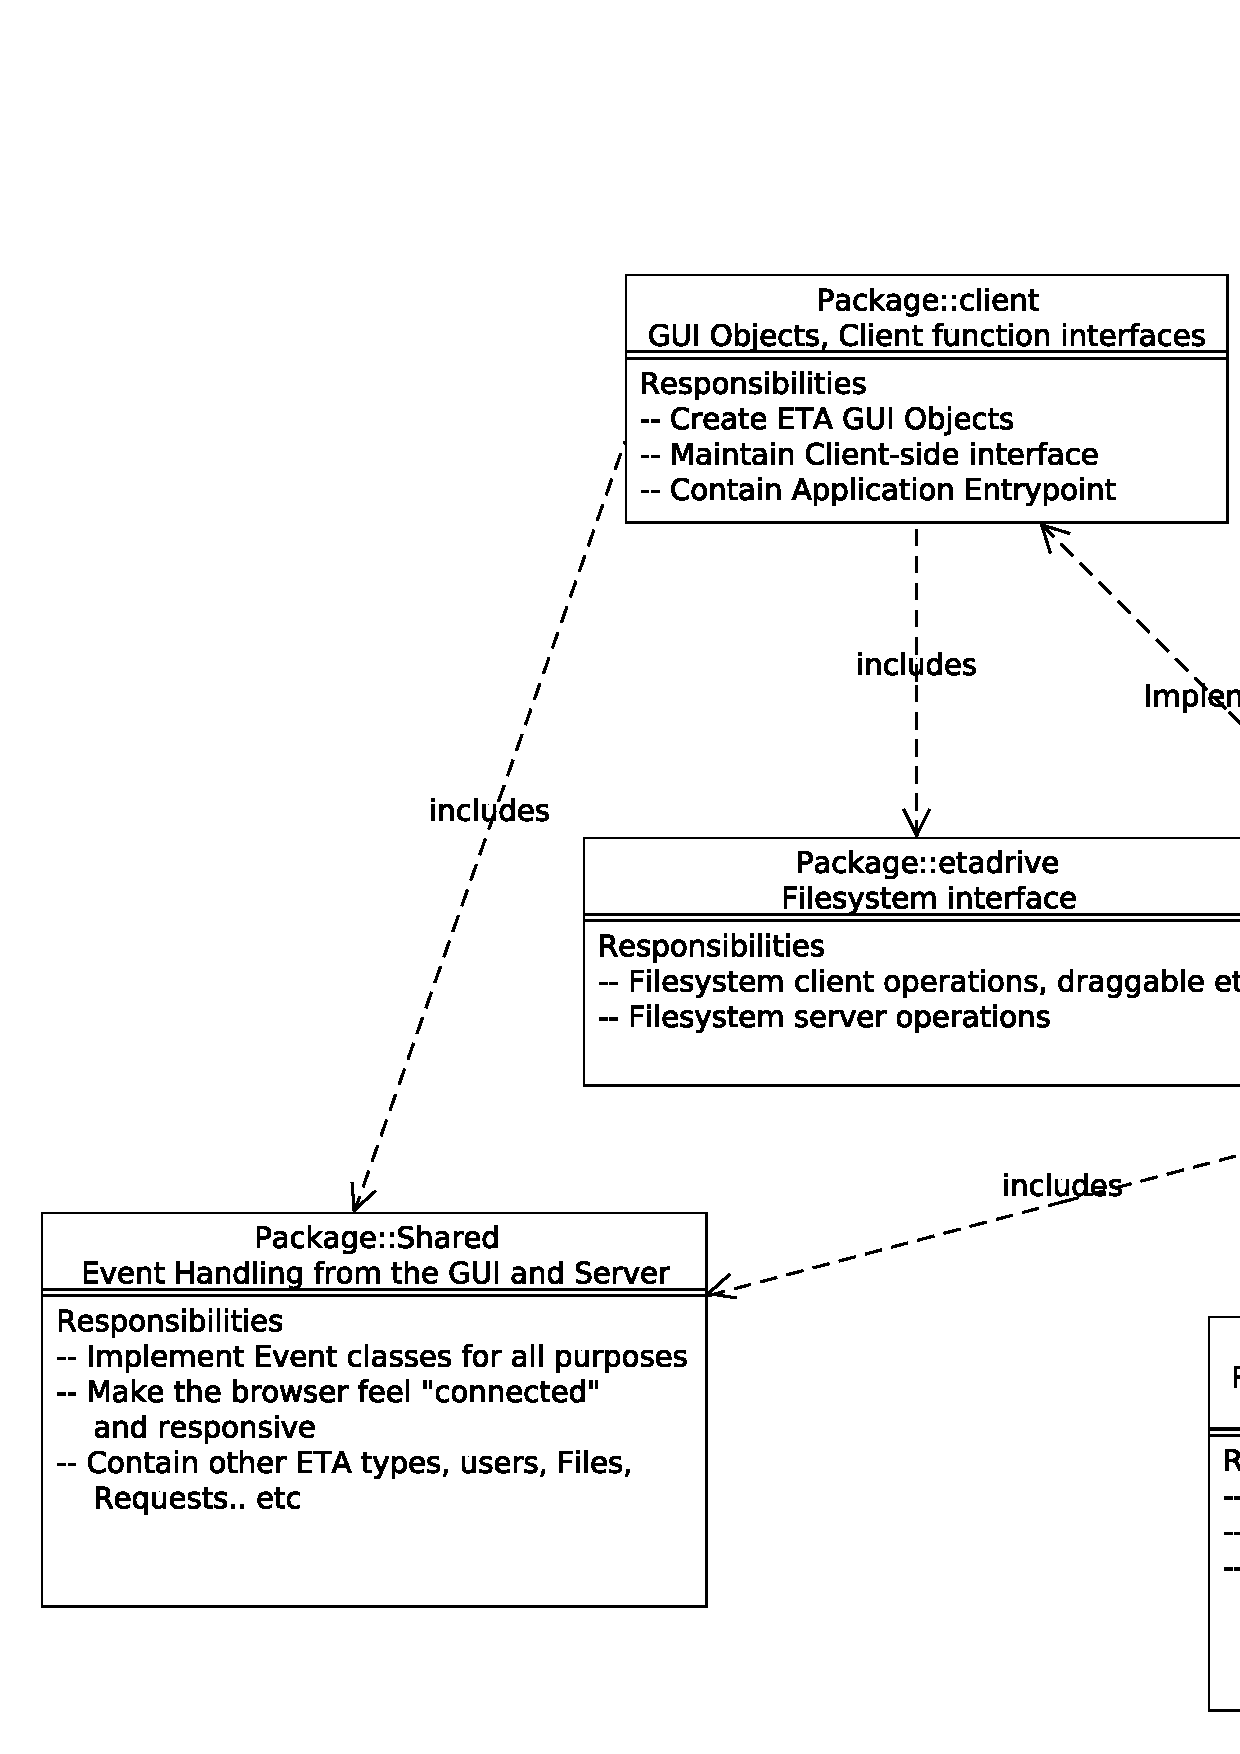
\includegraphics[width=1\textwidth]{ETAPackageOverview.jpg}
\caption{UML Diagram: ETA Package Overview}
\label{fig:ETAPackageOverview}

\end{figure}
\newpage
\section{Outline}
\begin{outline}
\item {\bf Introduction }
	\begin{outline}
	\item { Need and Purpose, how research is done, who needs it, etc.} \\
	\item { "What is" Easy-Terminal-Alternative } \\
	\item { Benefits}
	\end{outline}
\item {\bf Architecture}
	\begin{outline}
	\item { Technologies} \\	
	\item { AO Design Decision} \\
	\item { Package Overview} \\
	\item { Dataflow Overview and Diagrams} \\
	\item { Environment (Linux Environment)} \\
	\end{outline}
\item {\bf Installation}
	\begin{outline}
	\item { System Dependencies } \\
	\item { Downloading the source} \\
	\item { Configuring the source } \\
	\item { Building the source} \\
	\item { Launching the application} \\
	\end{outline}
\item {\bf Extension and Formal Documentation}
	\begin{outline}
	\item { Auth service example} \\
	\item { Job service example} \\
	\item { Modifying Client example}\\
	\item { Java-docs} \\
	\end{outline}
\item {\bf Conclusion}
	\begin{outline}
	\item { Current state of ETA} \\
	\item { Future Work, unit-tests, auto install} \\
	\end{outline}
\end{outline}





\setlength{\parindent}{0.5in}
 
\begin{workscited}

  \bibent
 Ambra Molesini, Alessandro Garcia, Christina von Flach Garcia Chavez, Thais Vasconcelos Batista, Stability assessment of aspect-oriented software architectures: A quantitative study, Journal of Systems and Software, Volume 83, Issue 5, May 2010, Pages 711-722, ISSN 0164-1212, 10.1016/j.jss.2009.05.022.
\\http://www.sciencedirect.com/science/article/pii/S0164121209001162. 

 \bibent
 "Apache Tomcat 6.0." \textit{Tomcat Documentation Index}. 9 Oct. 2012. Apache Foundation.  13 May 2013 http://tomcat.apache.org/tomcat-6.0-doc/. 

 \bibent
 "Google Web Toolkit." \textit{Developer's Guide}. 26 Oct. 2012. Google. 13 May 2013 \\https://developers.google.com/web-toolkit/doc/latest/DevGuide. 

 \bibent
 "Java Platform SE 7." \textit{Java Platform SE 7}. 28 July 2011. Oracle Inc. 13 May 2013 http://docs.oracle.com/javase/7/docs/api/. 


 \bibent
  Schroder, Carla. "Linux Bug \# 1: Bad Documentation" \textit{The Many Faces of Documentation}. N.p., 17 Nov. 2009. Web. 13 May 2013.\\ http://www.linuxplanet.com/linuxplanet/reports/6904/1/. 


 \end{workscited}

\end{document}